\chapter{Introduction}\label{chap:Introduction}

\section{Background}

Biological sequences, including nucleotide sequences (DNA and RNA) and peptide sequences (proteins), play an fundamental role in life and reproduction. A nucleotide sequence consists of a chain of linked nucleotide bases. There are four possible types of bases in a DNA sequence, represented by four letters A, T, G, and C. A peptide sequence consists of linked amino acids, which have 20 different common types. Figure \ref{tab:code-dna} and \ref{tab:code-aa} shows their notation rules recommended by the International Union of Pure and Applied Chemistry (IUPAC) \cite{Cornish-Bowden:1985lr}.

\begin{table}[hbt]
\centering\small
\caption{IUPAC Nucleotide Notation Rules}\label{tab:code-dna}
\begin{tabular}{cc} \toprule
  IUPAC Code  & Base                \\ \hline
  A           & Adenine             \\
  C           & Cytosine            \\
  G           & Guanine             \\
  T (or U)    & Thymine (or Uracil) \\
  N           & any base            \\
  . or -      & gap                 \\ \bottomrule
\end{tabular}
\end{table}

\begin{table}[hbt]
\centering\small
\caption{IUPAC Amino Acid Notation Rules}\label{tab:code-aa}
\begin{tabular}{ccc} \toprule
  IUPAC Code  & Three Letter Code & Amino acid    \\ \hline
  A           & Ala               & Alanine       \\
  C           & Cys               & Cysteine      \\
  D           & Asp               & Aspartic Acid \\
  E           & Glu               & Glutamic Acid \\
  F           & Phe               & Phenylalanine \\
  G           & Gly               & Glycine       \\
  H           & His               & Histidine     \\
  I           & Ile               & Isoleucine    \\
  K           & Lys               & Lysine        \\
  L           & Leu               & Leucine       \\
  M           & Met               & Methionine    \\
  N           & Asn               & Asparagine    \\
  P           & Pro               & Proline       \\
  Q           & Gln               & Glutamine     \\
  R           & Arg               & Arginine      \\
  S           & Ser               & Serine        \\
  T           & Thr               & Threonine     \\
  V           & Val               & Valine        \\
  W           & Trp               & Tryptophan    \\
  Y           & Tyr               & Tyrosine      \\ \bottomrule
\end{tabular}
\end{table}

Since the 1970s, sequences of more than 160,000 organisms have been decoded and analyzed by researchers \cite{Benson:2007lr}. With the explosively growing amount of data, it is impractical to study sequences manually. Computer-aided techniques are needed to help analyze their structures, functions and evolution.

Multiple sequence alignment (MSA) is one of the computational ways to identify regions of similarity between sequences and is required by almost all comparative sequence studies. An MSA is typically organized as a matrix, in which each row represents a sequence, and each column corresponds to an hypothetically equivalent position across all the sequences aligned. Each element of the matrix contains a symbol, which can be either `-' (a gap) or a sequence symbol (a nucleotide base for DNA/RNA sequences, or an amino acid for protein sequences) \cite{Edgar:2006aa}.

\begin{figure}[hb]
\scriptsize
\begin{verbatim}
  AY169803.O  MHYRDLSTLIIVSALLLINVXLWMFILRXYLEHKRQERREREILERLRRIREIKDDSDYESNGEEEQEVMD-LVHSHGFDNPMFEL
  AY169809.O  MQYKGL--LLIIIALLLINVXVWMFNLRKYLEQKKQERREREVINRLRRIREVKDDSDYESNGEEEQEVME-LVHSHGFDNPMFEL
  AY169807.O  MLHRDLLLLIIISALLLTNIILWMFVLRKYLEIKKQERREREILERLRXIREIRDDSDYESNEEEEQEVRDHLVHTFGFANPMFEI
  AY169811.O  MHHRDLLTLIAVSALLFINIILWIYVLRKYLEQRKQDRREREILERLRRIXEIGDDSDYESNEEEEQEVMD-LVHNHGFDNPMFEP
  AJ302646.O  MHHRDLLALITTSALLLTNVVLWTFILRQYLKQKKQDKREREILERLRRIRQIEDDSDYESDGTEEQEVRD-LVHSYGFDNPMFEL
  AY169815.O  MQHKDLLILIITSALLLINVILWLFVLKQCLEQKKQTKREREIIRRLRRIREIEDDSDYESNGEEEQTVRD-LIHSHGFDNPMFEL
  AY169804.O  MHQRDLLILIAVSILCLICILVWTFNLRKYLEHRKQDKREREILERLRRVREIRDDSDYESBGEEEQEVMD-LIHSHGFANPLFEL
  AY169810.O  MNYKELLSLIVVSVLLLAAIVIWMFILKKYLEQKEQDRRERELLKRIERLXEXRDDSDYESNGDEEQEVMH-LVHTHGFANPMFEL
  AY169806.O  MYKDQIILIIIFCVVFLIAACIWLFILKTYLEQKKQDRREKELLRRLQRIIEIRDDSDYESNGEEEQEVMD-LVHEHGFVNPMFEL
\end{verbatim}
\caption[Example of Multiple Sequence Alignment]{An example of multiple sequence alignment, generated by \emph{ClustalW} \cite{Thompsonaa}. Each row in the MSA represents one protein sequence. The leftmost column shows sequence names. The right part is the alignment matrix.}\label{fig:msa}
\end{figure}

An MSA result can be a large and complex matrix. To highlight similarity or other properties, certain visualization methods are applied. Some alignment programs, like ClustalW, add an asterisk, colon, semicolon, or other symbols, to show conservative columns. Some others use color to display information: assign each nucleotide or amino acid its own color, and indicate amino acid properties with an empirical color assignment. Figure \ref{fig:procter-2a} shows a protein MSA colored using Jalview \cite{Waterhouse:2009fk}.

\begin{figure}[hbt]
\center{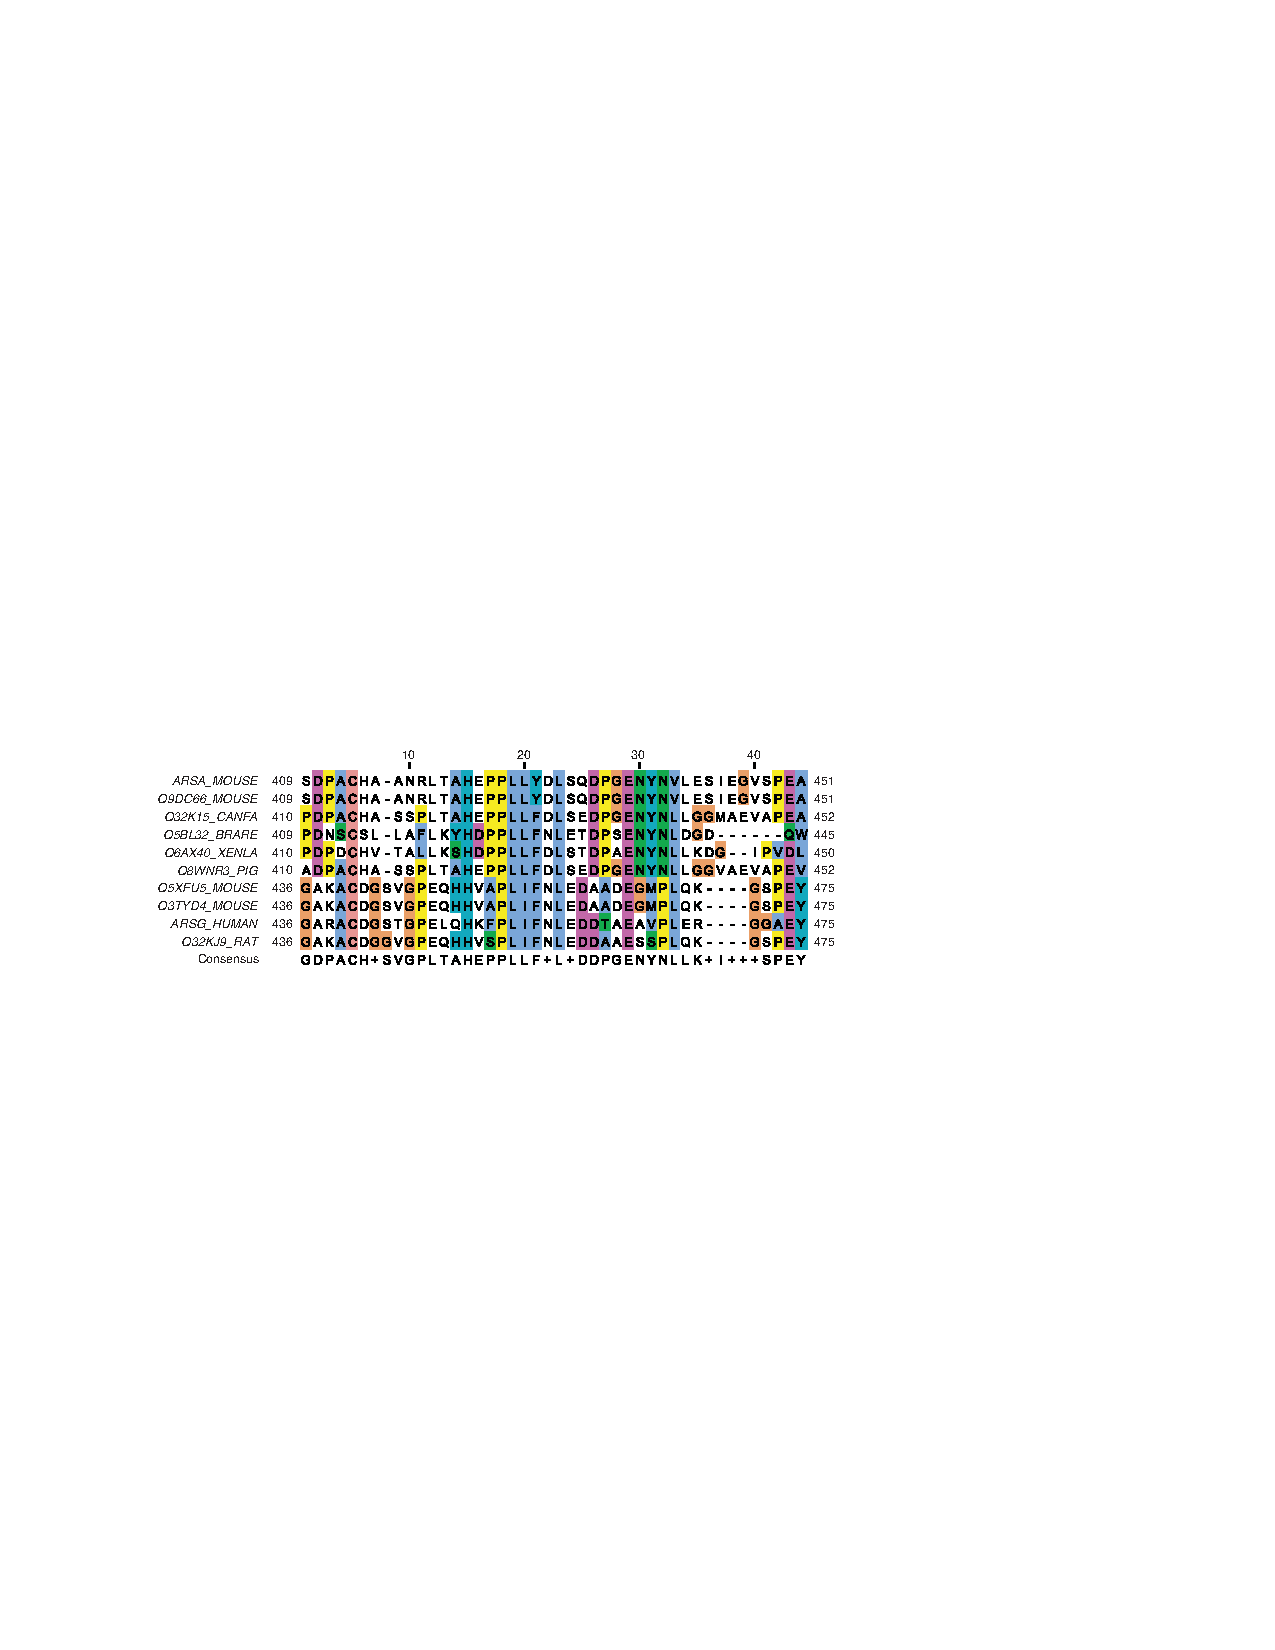
\includegraphics[width=0.9\textwidth]{figures/procter2a.pdf}}
\caption[Protein MSA Colored with Jalview]{A protein MSA colored with Jalview \cite{Waterhouse:2009fk,Procter2010aa}.}\label{fig:procter-2a}
\end{figure}

\section{Related Work}

Numerous MSA visualization applications, either stand-alone or web-based, have been developed in recent decades, ranging from simple MSA viewers, to complex editing and analysis platforms. Many of them have graphical user interfaces showing a grid of symbols, usually along with various colorings, sizings and annotations \cite{Procter2010aa}.

\begin{figure}[hbt]
\centering
\subfloat[Some nucleotide color schemes.]{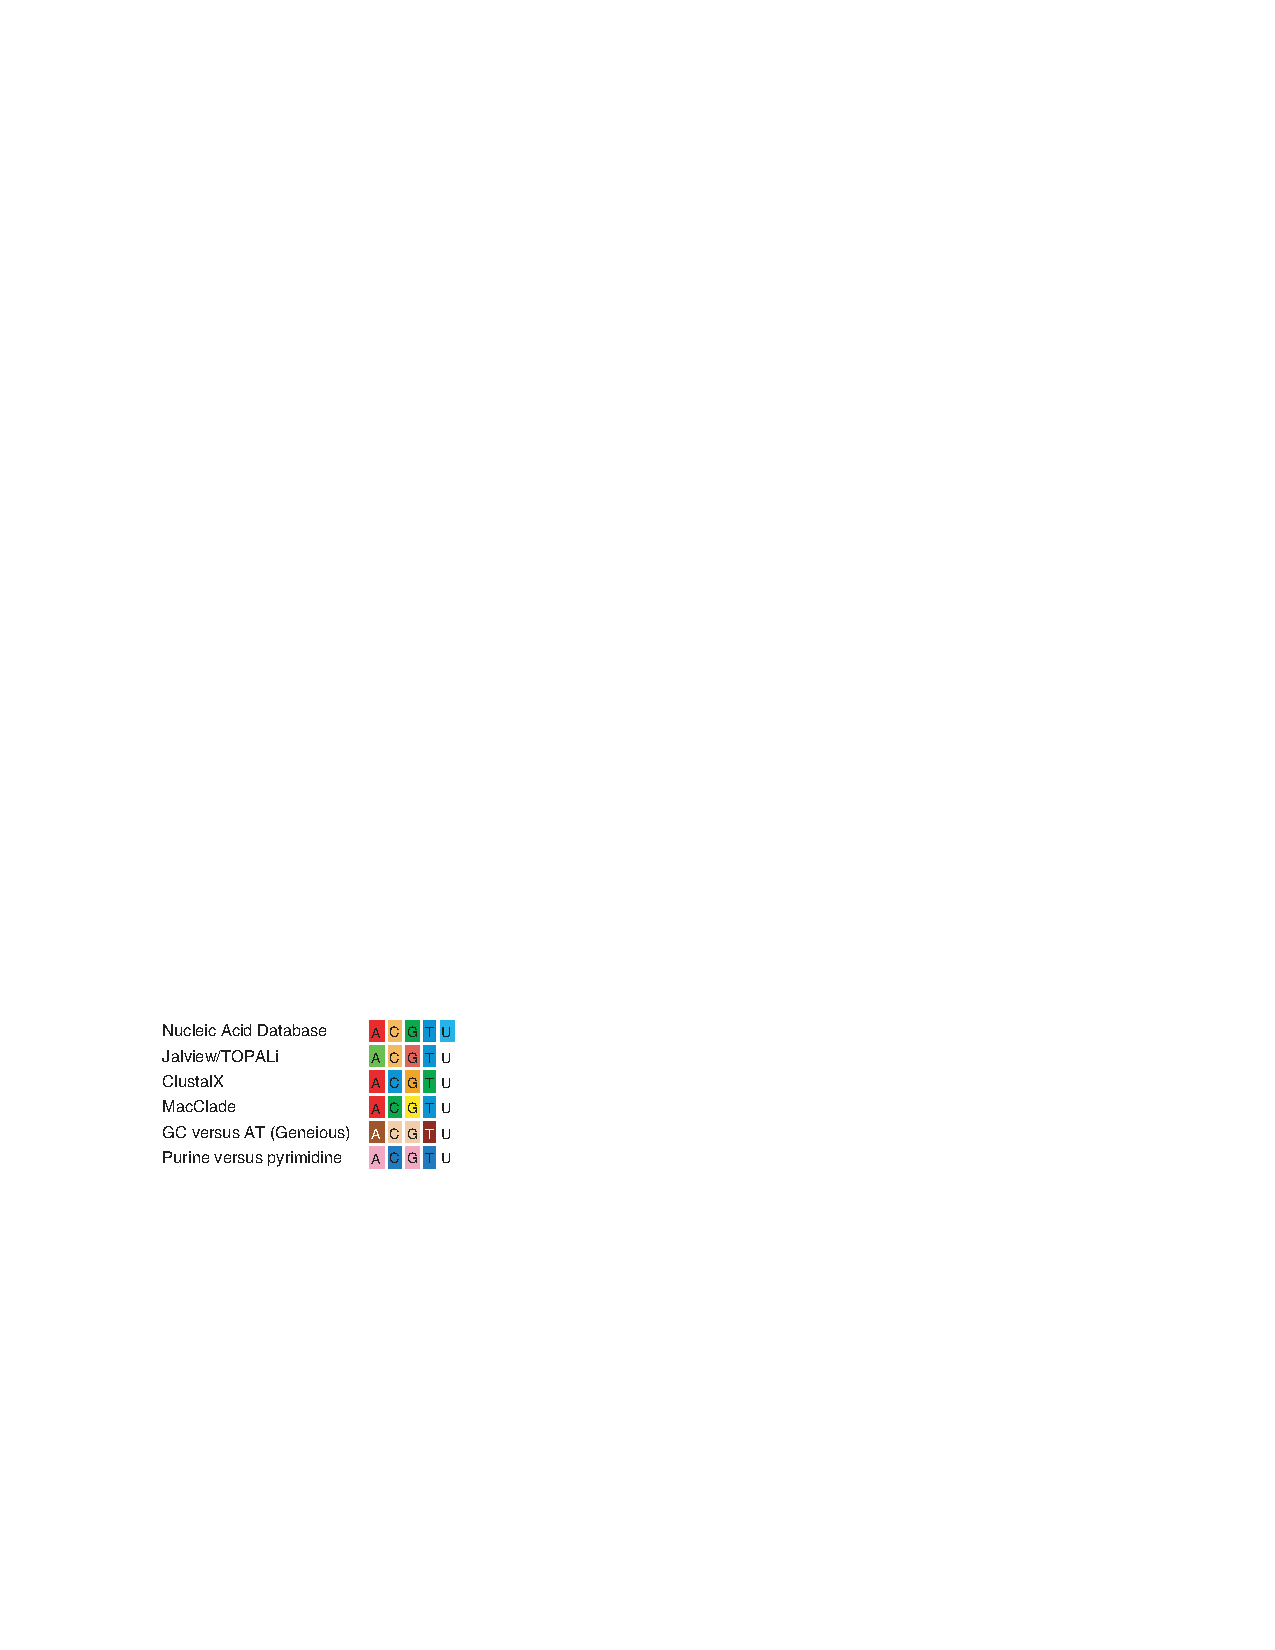
\includegraphics[width=0.4\textwidth]{figures/procter2c.pdf}}
\subfloat[Some amino acid color schemes.]{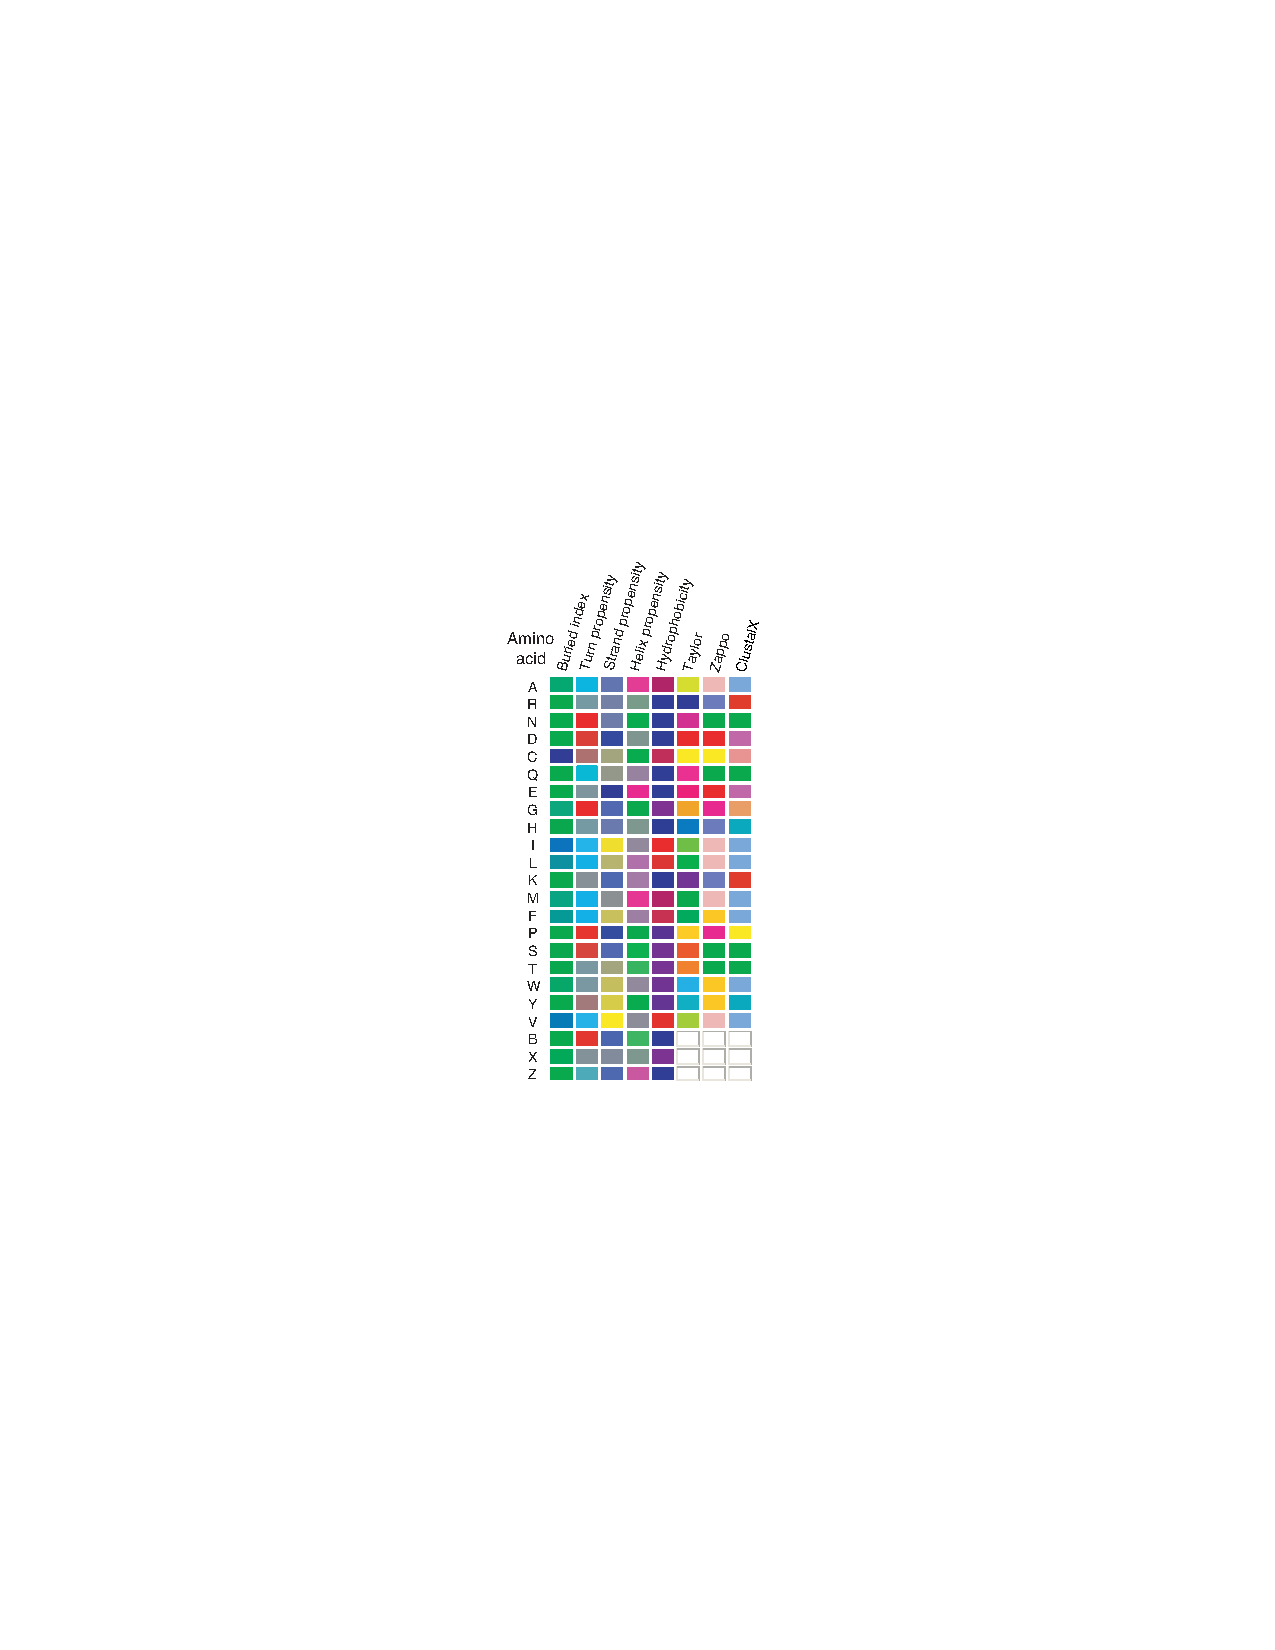
\includegraphics[width=0.4\textwidth]{figures/procter2b.pdf}}
\caption[Some Nucleotide and Amino Acid Color Schemes]{Examples of color schemes used by some visualization tools \cite{Procter2010aa}.}\label{fig:procter-2bc}
\end{figure}

Coloring an alignment has been widely implemented to highlight specific regions, properties, or patterns. For example, sequences can be colored according to the similarity to consensus sequence, physicochemical properties of amino acids, or secondary structure of the proteins.

The simplest way of coloring is to use a fixed color scheme, in which each sequence symbol has its own color, and will not be changed across the alignment. The assignment of color schemes are usually based on some empirical properties or chemical classifications. Figure \ref{fig:procter-2bc} shows some nucleotide and amino acid color schemes used by major visualization tools.

Numerous color schemes are available for different purposes. Taylor \cite{LIN2002361} and Clustal \cite{Thompsonaa} are two of the most frequently used and often considered \emph{de facto} standards. Figure \ref{fig:procter-2d} shows Taylor's Venn diagram of color scheme.

\begin{figure}[hbt]
\center{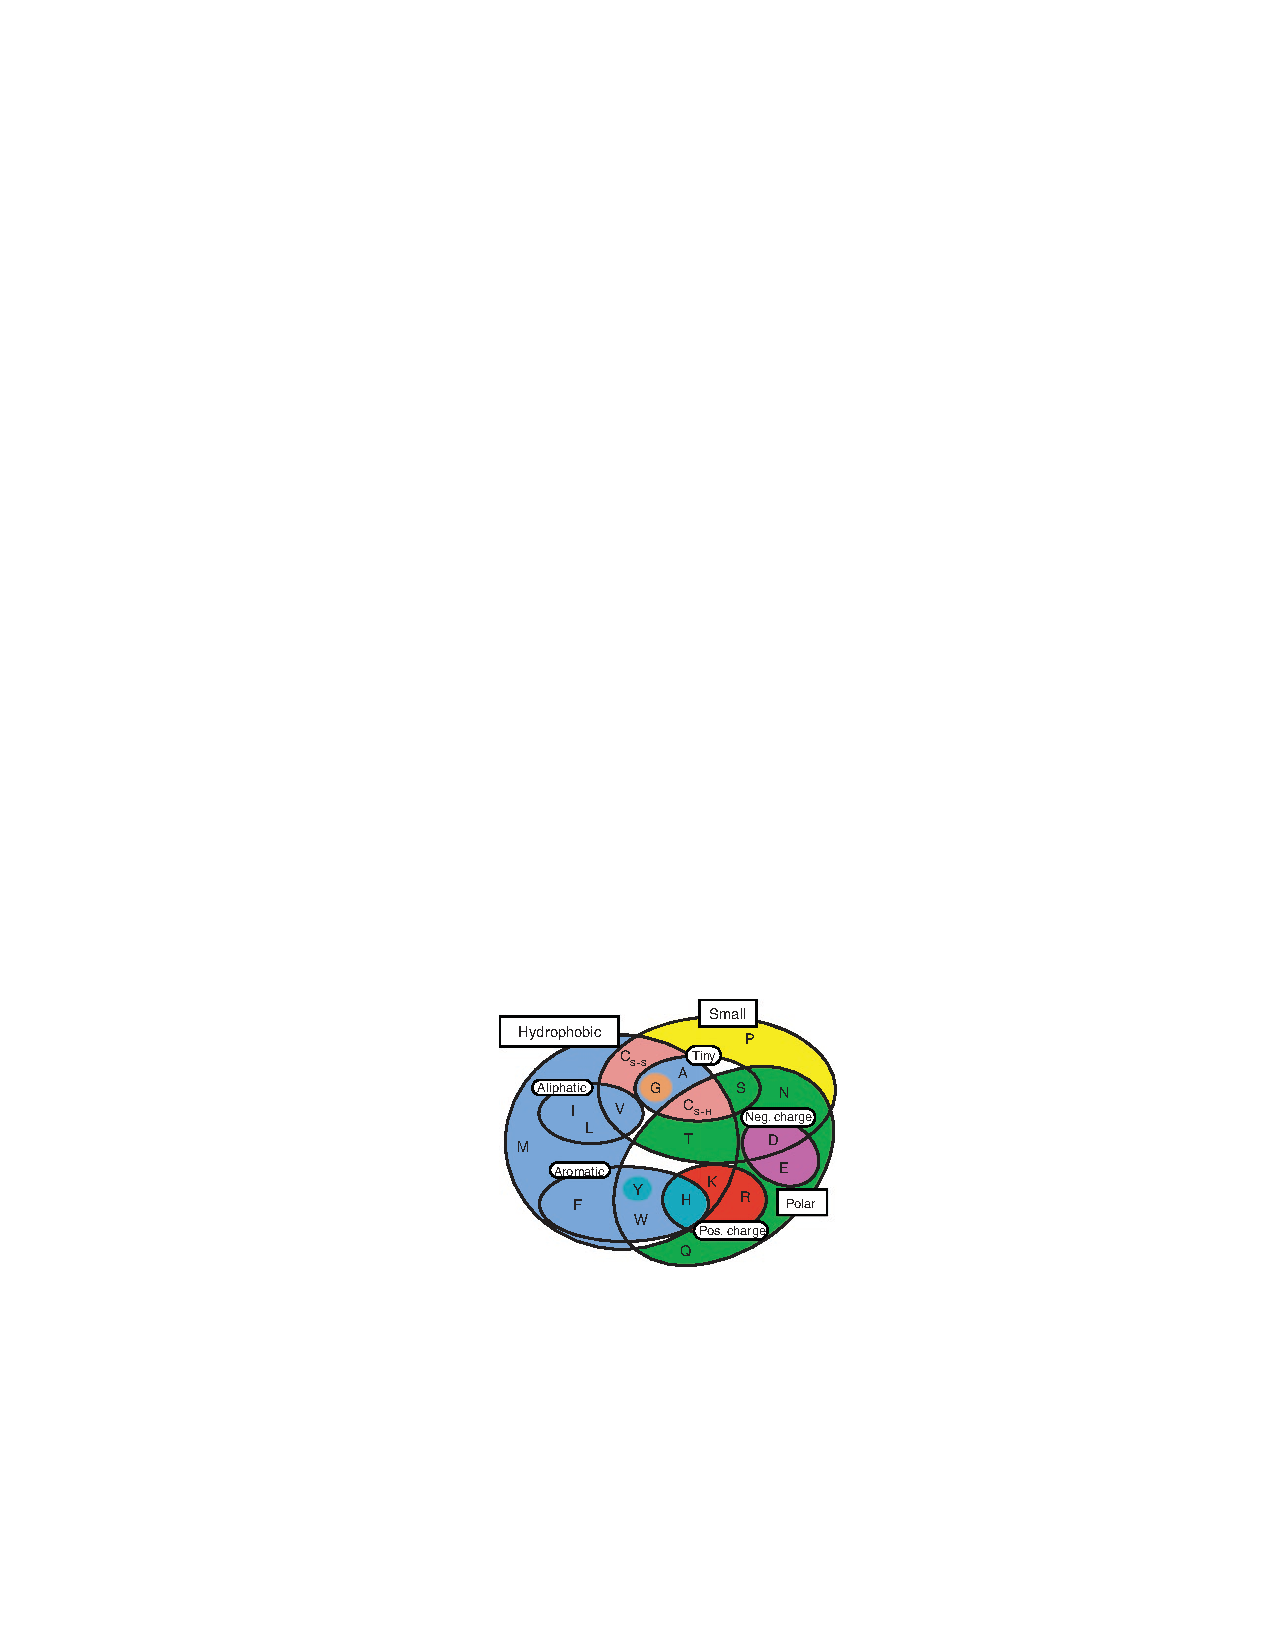
\includegraphics[width=0.6\textwidth]{figures/procter2d.pdf}}
\caption[Taylor's Amino Acid Color Scheme]{Taylor's \cite{LIN2002361} Venn diagram showing the color scheme based on the physicochemical properties of the amino acid groups \cite{Procter2010aa}.}\label{fig:procter-2d}
\end{figure}

Using these pre-determined color schemes to color sequence symbols, however, is not always helpful for phylogenetic analysis. Those fixed color schemes reflect chemical differences between specific types of symbols, rather than between sequences, regions, blocks, or structures of the alignment.

When symbols are examined within one column, the colors successfully show the similarities. But in the horizontal aspect, comparative information within a row or a rectangular region are unable to be displayed. For example, how is one sequence similar to others? Which sections align better than others? Which areas of the alignment are more conserved? How robust is the alignment accuracy?

To make things worse, fixed color scheme can introduce confusions. Color difference between different columns gives an impression of dissimilarity, while it actually represents nothing. Figure \ref{fig:intro1} shows an example of this confusion.

\begin{figure}[hbt]
\centering
\subfloat[A perfectly aligned MSA. However, the color graph is distractive and fails to convey a `perfect' feeling.]{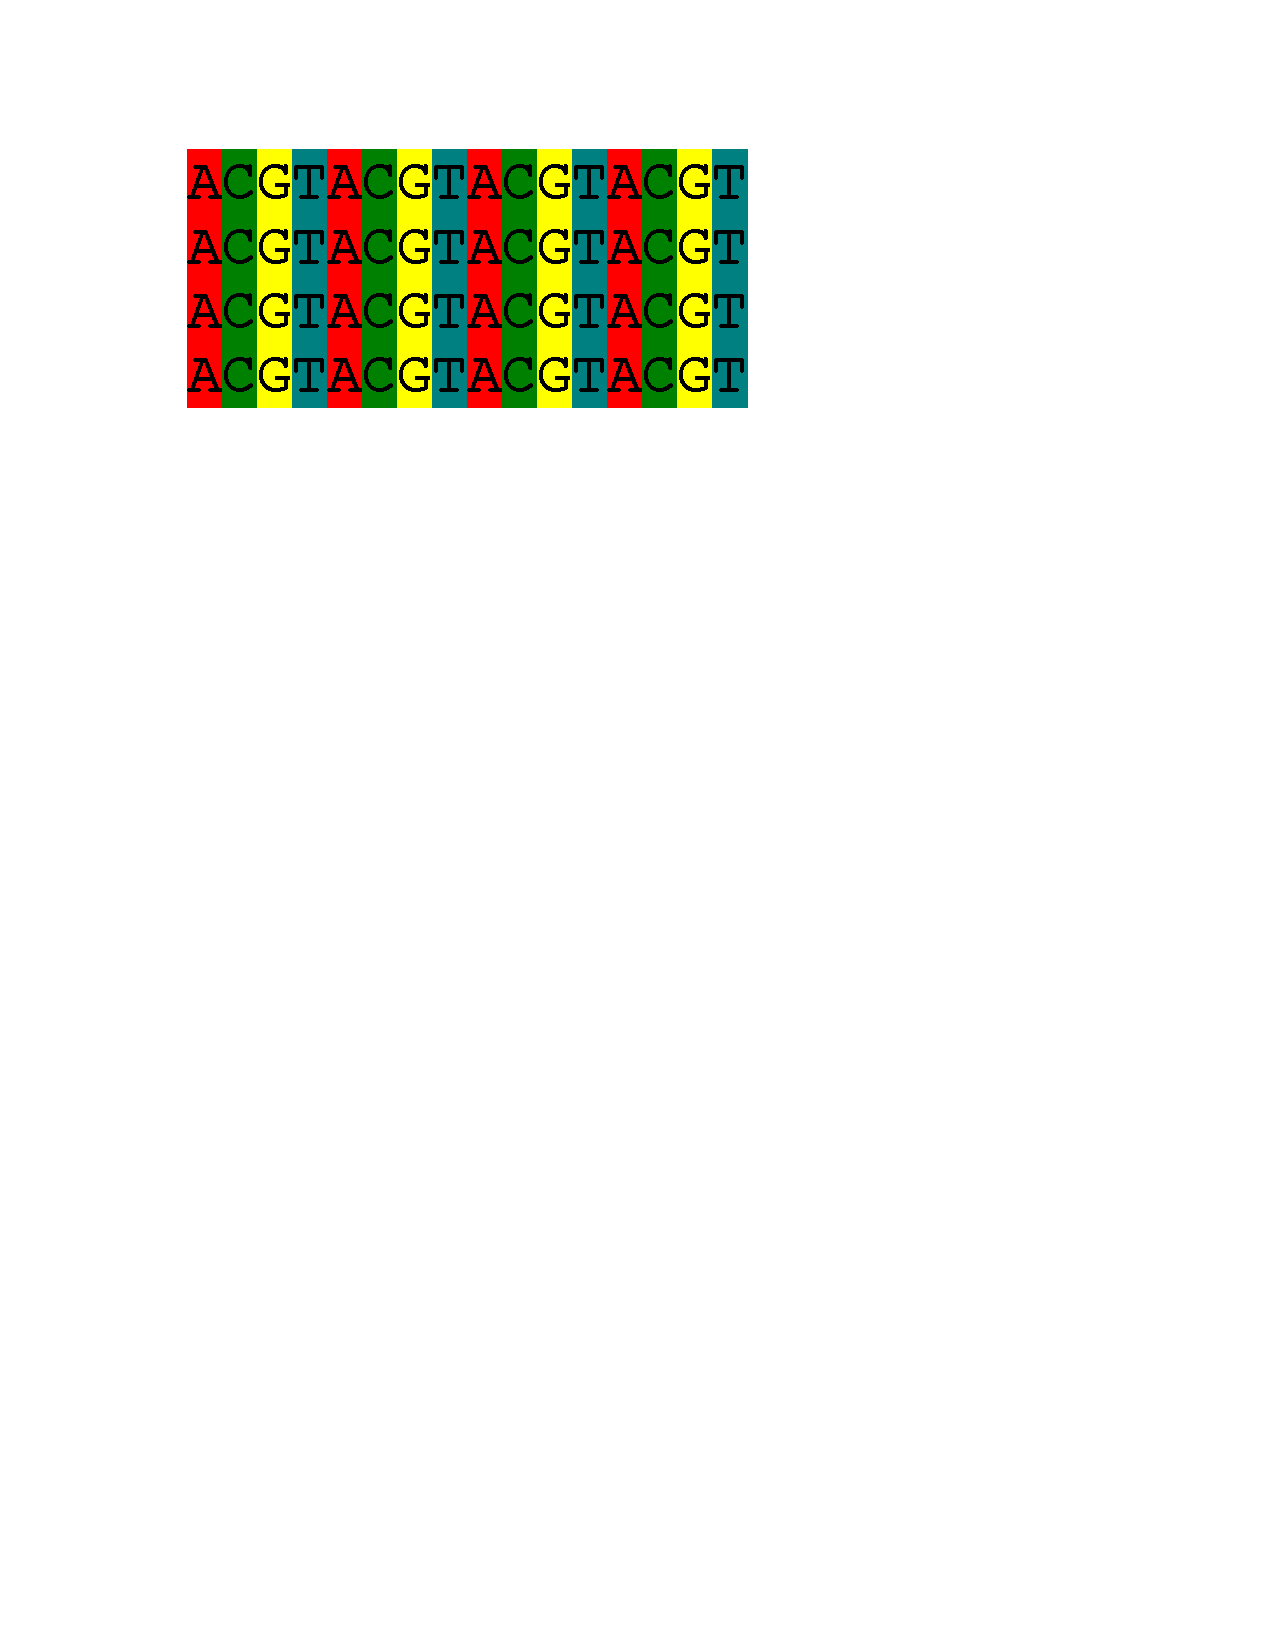
\includegraphics[width=0.35\textwidth]{figures/intro1.pdf}}
\hspace{5mm}
\subfloat[This is an extremely poorly aligned one, but the color graph looks even better than (a).]{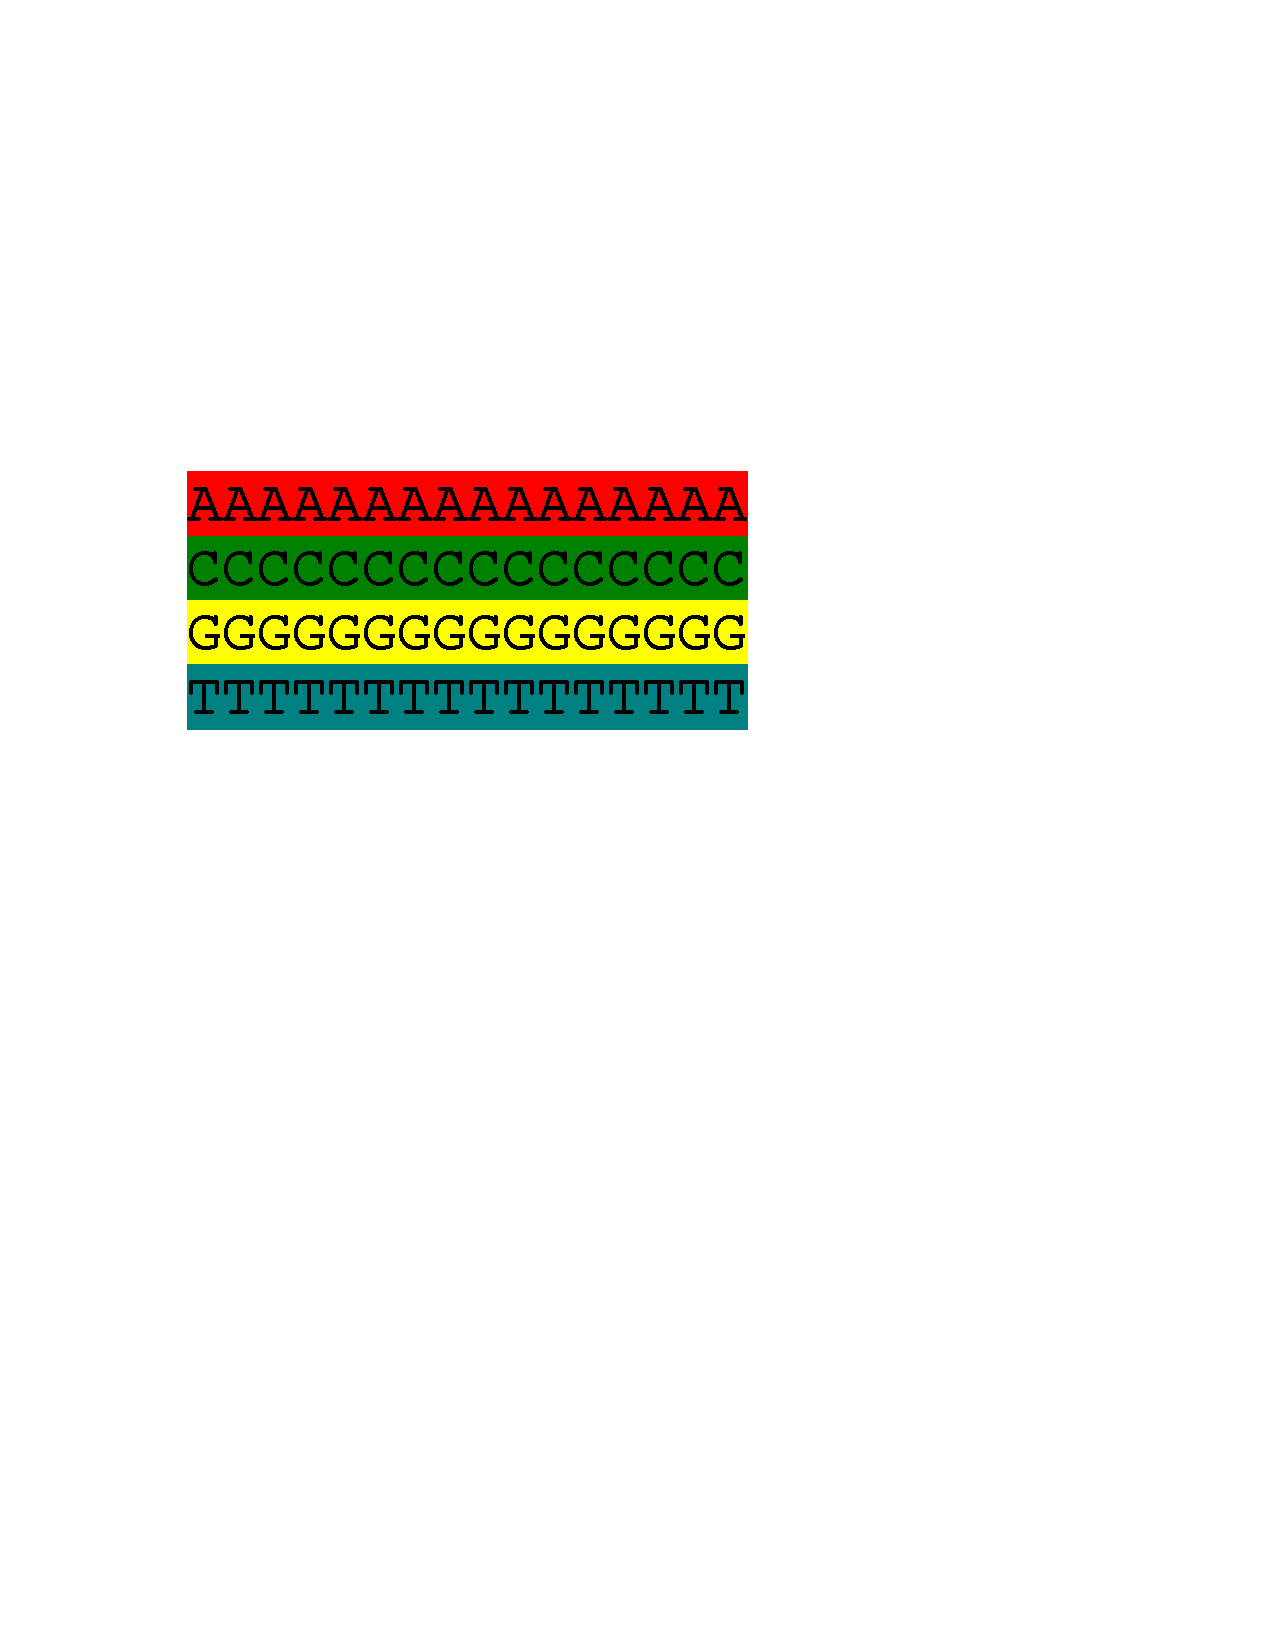
\includegraphics[width=0.35\textwidth]{figures/intro2.pdf}}
\caption[Fixed Color Scheme Introduces Confusion]{Fixed color scheme introduces confusions.}\label{fig:intro1}
\end{figure}

\section{Thesis Outline}

In this report, we introduce a new MSA visualization tool called \emph{Mavis} (Multiple Alignment VISualization). Mavis focuses on highlighting evolutionary relationships and internal structures of an alignment. Instead of relying on chemical properties or any other information from specific symbol types, our approach is based on only one metric, which is the symbol-symbol similarity score. The color of a sequence residue will not depend on its symbol type, but on its similarity scores with other residues. By applying this new approach, we are able to provide a big picture of an MSA, in which the structure and quality are clearly displayed.

The rest part of this thesis is organized into five chapters. Chapter 2 explains the general idea of how Mavis is designed and the steps it takes to color an MSA on a high level. Chapter 3 expounds the core algorithm step by step, from multidimensional scaling, to color mapping, and to optimization. Chapter 4 describes the implementation of the algorithm, including the back-end, API, and different user interfaces. Chapter 5 presents some test results to show the validity and performance of our implementation. The entire study is discussed in Chapter 6 and concluded in Chapter 7.

The source code of Mavis back-end, API, and web interface is available in the Appendix at the end of this report.
